\section{Introduction}

Science is aiming towards open and reproducible research. In gamma-ray astronomy, especially for ground-based imaging atmospheric Cherenkov telescopes (IACT), data and software have so far been mostly private to the collaboration operating the telescopes. The Cherenkov Telescop Array (CTA), the next generation of IACT, will be operated as an an open observatory, meaning that data and analysis softwares will be public at the end-user, science tools level. Momentum was thus given to the development of open data format and open-source software for gamma-ray astronomy, leading to synergies between experiments, ground based and space missions. 

Open source analysis tools for VHE γ-ray astronomy have emerged. They all meet on common ground of using FITS files for data transfer. The current IACTs (H.E.S.S., MAGIC and VERITAS) all use their own software based on the ROOT library, which makes it impossible to analyse the respective data with anything else than the corresponding software. Current open source analysis tools provide alternative analysis techniques compared to the present standard in VHE astronomy. It is assumed that these techniques (e.g. 3D likelihood analysis such as already implemented for Fermi-LAT) improve the sensitivity of IACTs by roughly 20\%. The data model for CTA is currently being developed but still work in progress. A main point of defining the high level data format for CTA is to understand the instrument including its systematics and IRF dependencies. In addition the needs from a user perspective have to be taken into account to create a solution as simple as possible. Having agreed on a common data format for files and on a way how to store and access those files (folder structure), makes mid-level (event energies, positions) and high-level (source position, morphology, spectrum) checks between the different chains, algorithms and open-source tools possible. This will also ease interoperability with other codes (e.g. to check results, combine results in one plot, ...). Currently two open-source science tools packages are being designed for current IACT and CTA data analysis, Gammapy (\cite{2015arXiv150907408D}) and Ctools (\citep{2016arXiv160600393K}). Gammapy is an in-development Astropy-affiliated package. Ctools is based on the GammaLib analysis framework, which is mainly written in C++.

We have created a  Github organization where we are developing high-level data format specifications, in accordance with astronomy standards. 

\section{How to contribute}

The specifications of a given data level format defines the names and semantics of data and header fields. Such specifications are made easy to understand. Specifications of this format are currently written that can form the basis for prototyping for data producers (mainly existing IACTs and simulated CTA data) and consumers (mainly science tool codes). We include example files and some explanations, in additon to the detailed specifications for a given format. 

The scope is high-level data, starting with event lists and instrument response functions (IRFs), what is called "data level 3" (DL3) in CTA. The first stable release (archived on Zenodo with a DOI) is coming soon.

If you want to contribute, it is simple:

\begin{itemize}
\item{}Use the existing format and give feedbacks. Propose additions and changes.
\item{}Join the mailing list (see next section). Send an e-mail with an idea or proposal.
\item{}Create a github account. File an issue with a correction or make a pull request proposing additions.
\end{itemize}

No formal approval process is in place yet as this is avery recent effort

\subsection{Resources}

\begin{itemize}
\item{}Mailing list for announcements and high level discussions (75 members, including people from all major gamma-ray collaborations : lists.nasa.gov/mailman/listinfo/open-gamma-ray-astro
\item{}Github issues and pull requests are used for detailed discussions: github.com/open-gamma-ray-astro
\item{}Data format specifications in HTML and PDF format, including example files : gamma-astro-data-formats.readthedocs.io/
\end{itemize}

\section{Format specifications content}

So far the focus has been mainly on the definition of the IACT DL3 formats.  A "general" section defines common things like details about time scales or coordinate systems. Some work on the definition of higher-level formats for spectra and lightcurves is on going. HEALPIX  (Hierarchical Equal Area isoLatitude Pixelization of a sphere) projection for images and  description of data cubes are also condidered.

Next sections will describe the effort toward the event list format definition as well as an example for spectra.

\subsection{IACT DL3}

DL3 format should describe all data released to the end users for analysis with science tools as , EVENT, IRF and TECH (technical data not directly attached to the object observed). Prototyping by existing IACTs (H.E.S.S.,MAGIC,VERITAS and science tools (GammaPy, Ctools) is a major activity. 

Many points are still under discussion/consideration:

\begin{itemize}
\item{}Observations modes, time intervals
\item{}How to link EVENET and IRF
\item{}Pointing and live time information
\item{}IRF axis and validity ranges
\item{}FoV coordinates
\end{itemize}

\subsection{Likelihood SED and light curves}

A format is developped to store spectral analysis results for exchange and publication, not only "flux points" and "upper limits", but also the full likelihood profiles. 

It was first developped in Fermipy (ref) and used for Fermi-LAT (ref). It is now being adopted by groung-based high energy astronomy. Likelihood profiles are important information when those data are to be used in global spectral energy distribution (SED) of a source. 

Description of light curves is another topic open for discussion. 

\begin{figure}[tb]
  \centerline{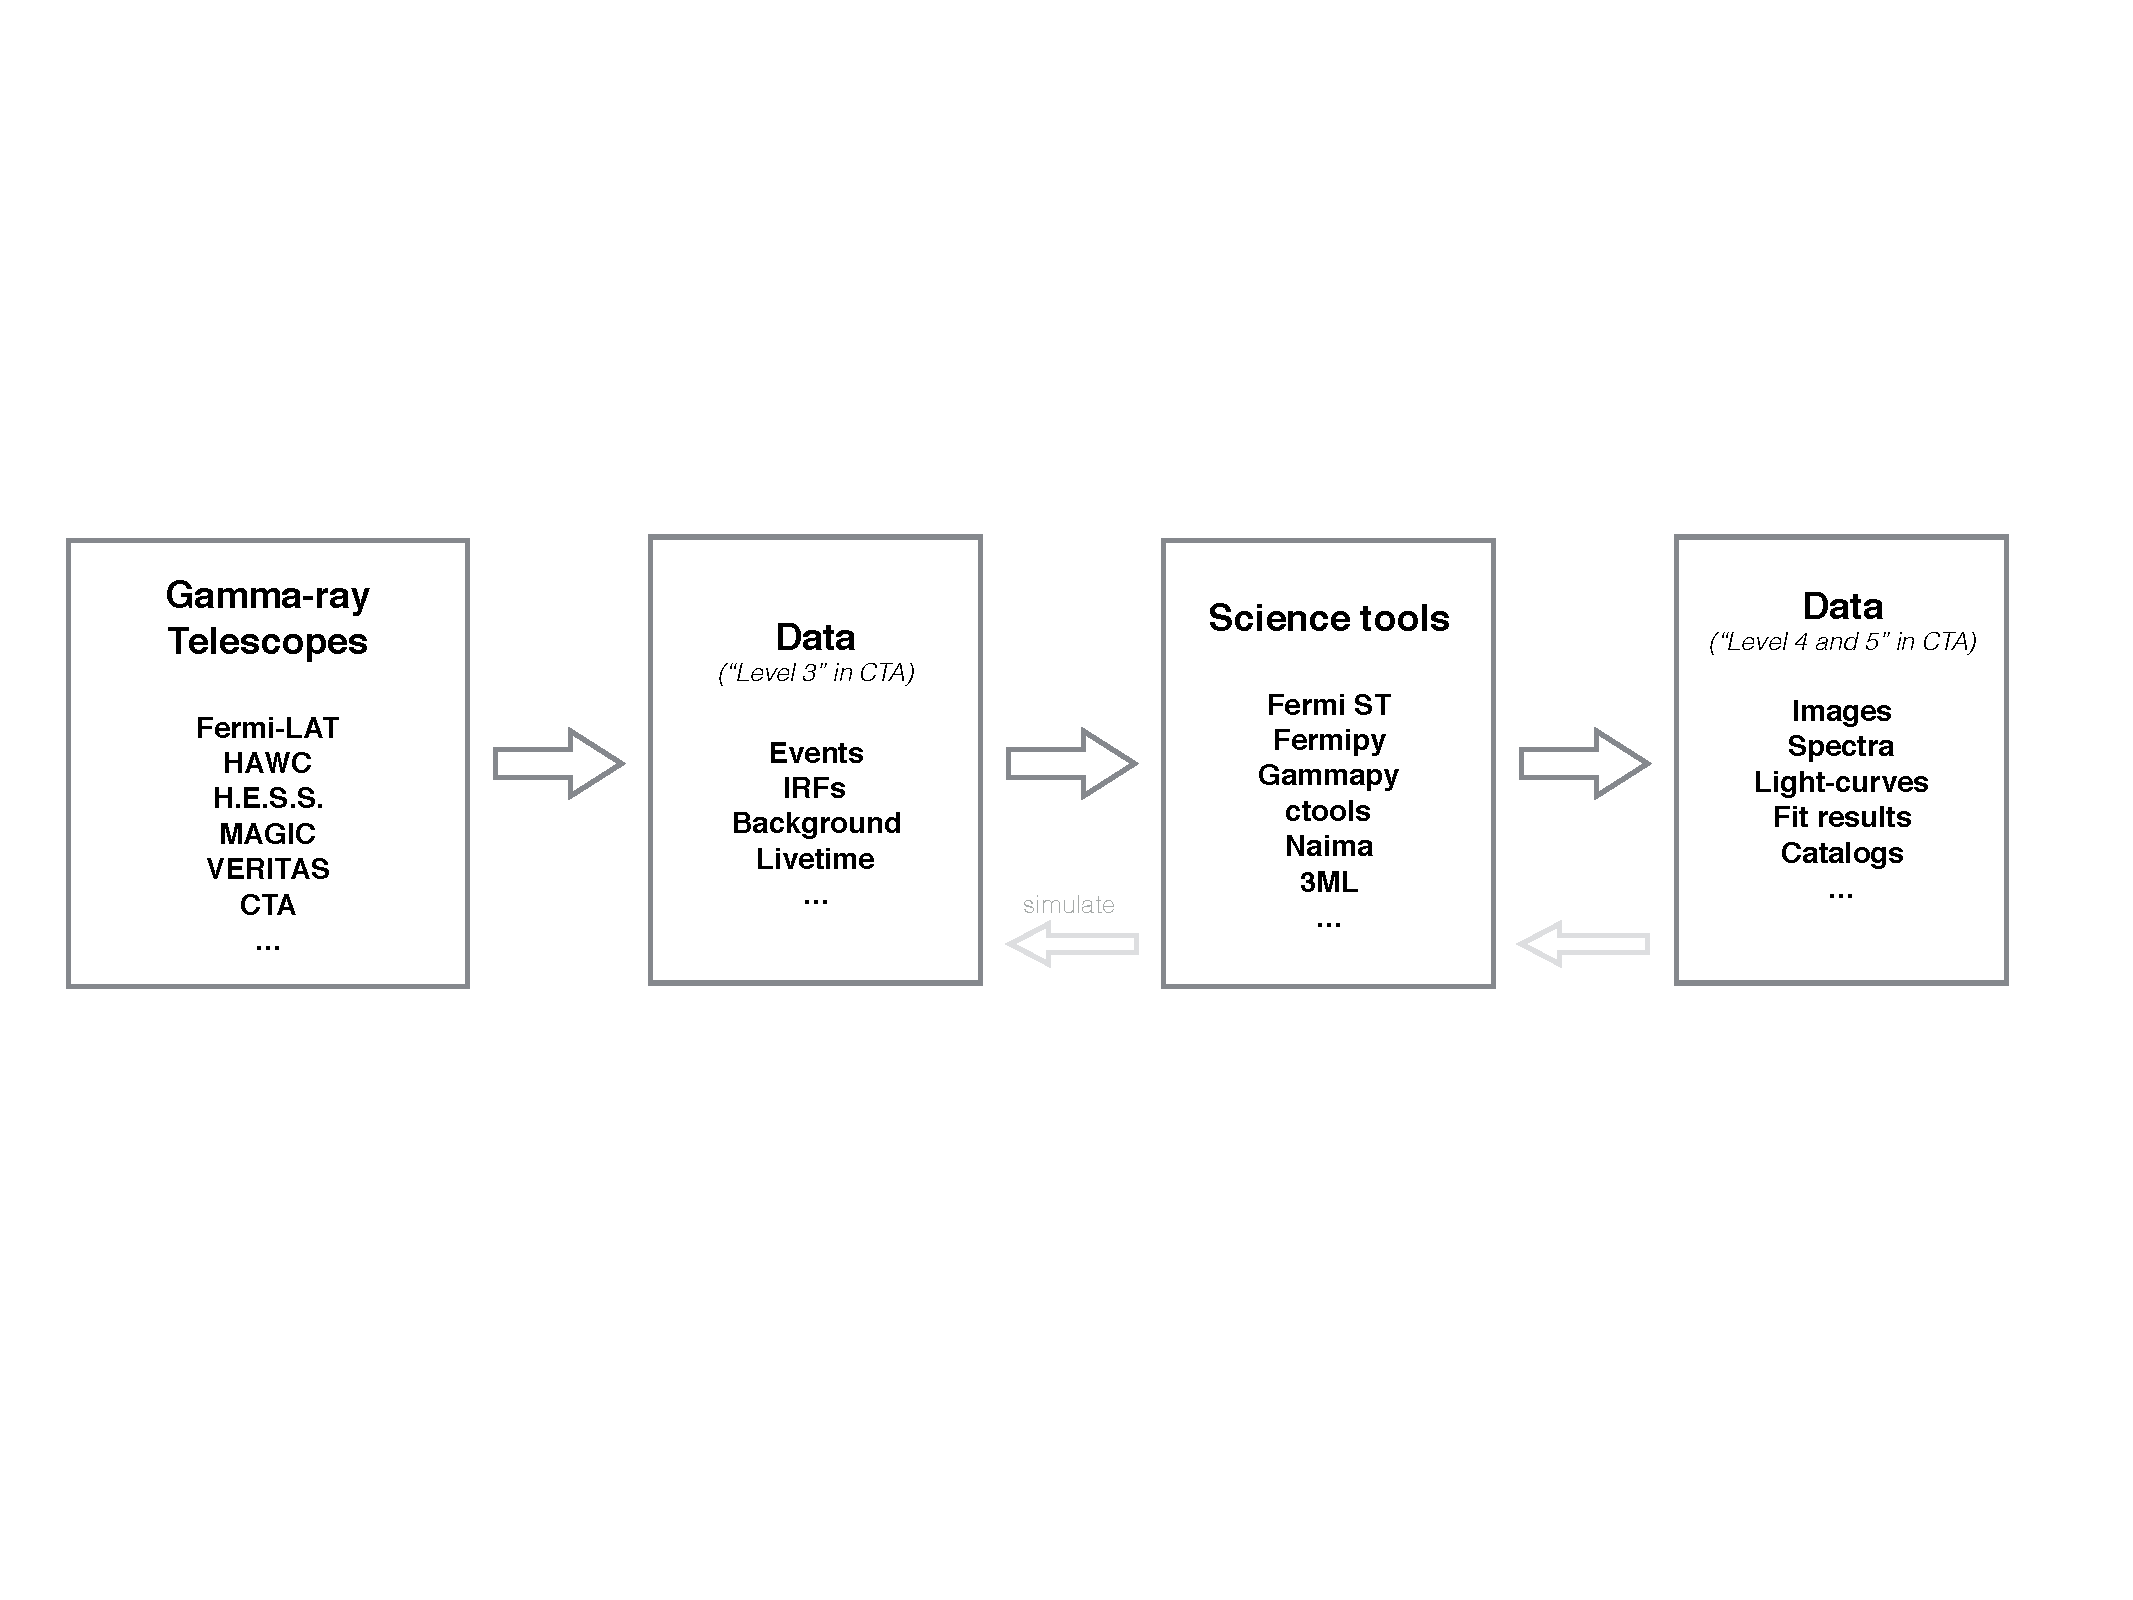
\includegraphics[width=\textwidth]{figures/purpose}}
  \caption{The purpose of the \texttt{gamma-astro-data-formats} effort: there's
  many gamma-ray data producers and consumers.}
\end{figure}

\begin{figure}[tb]
  \centerline{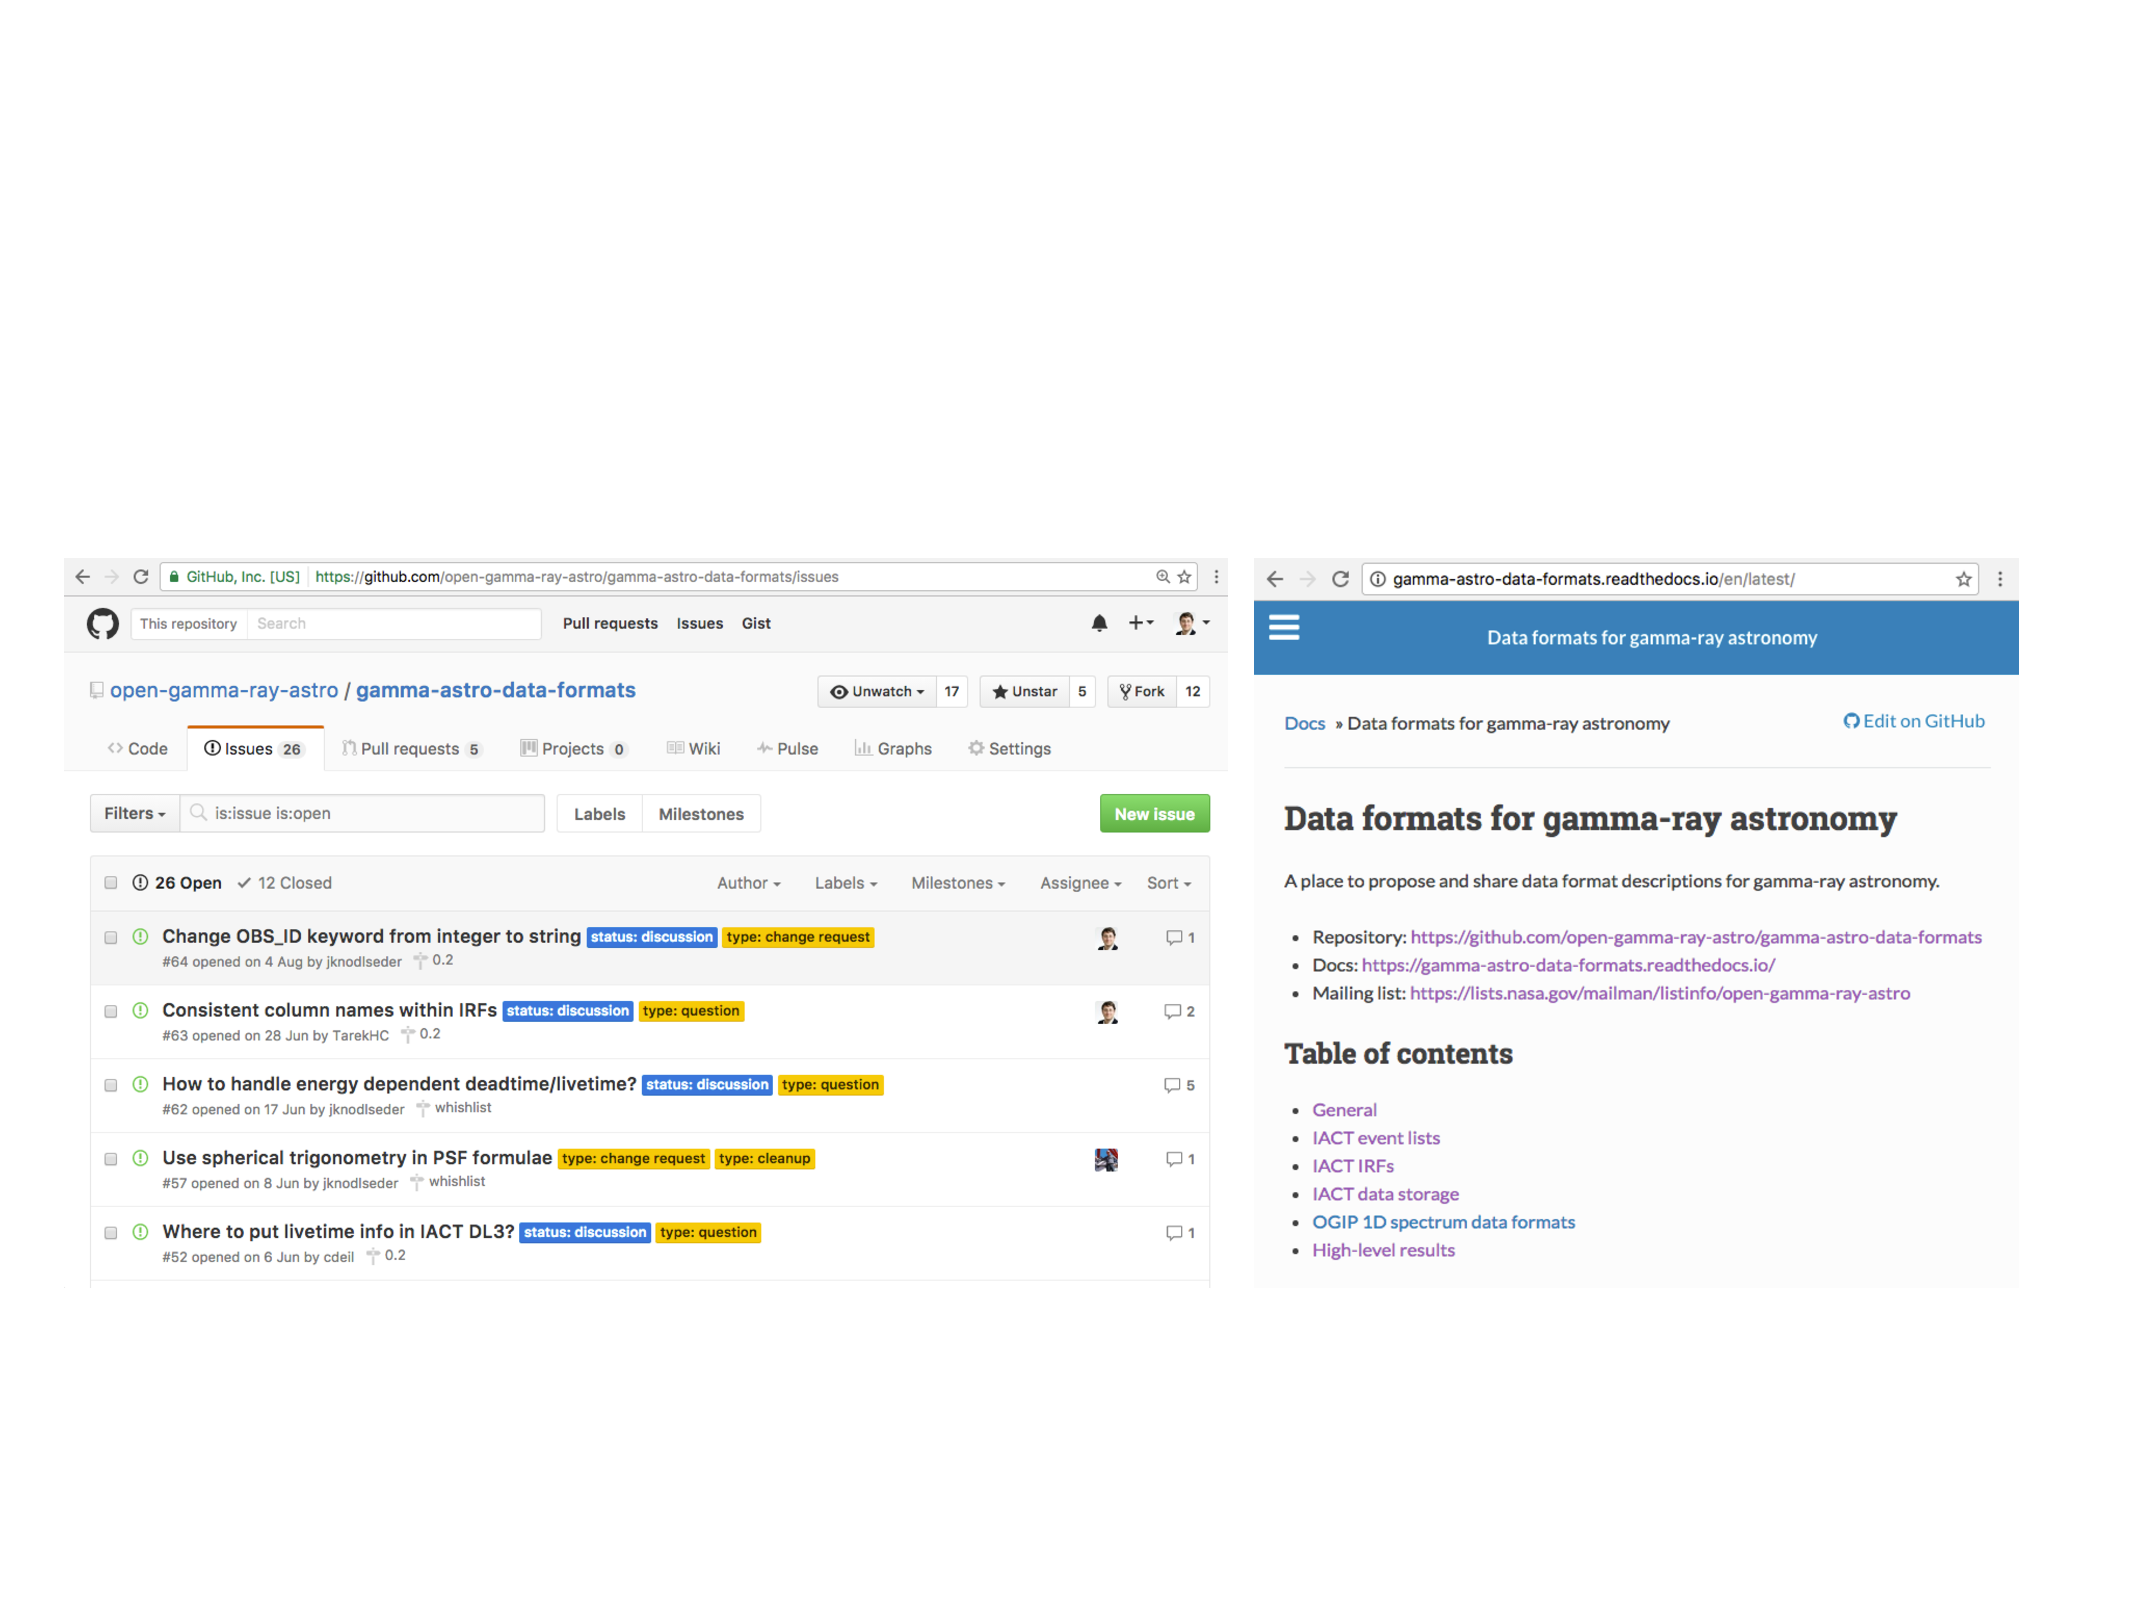
\includegraphics[width=\textwidth]{figures/webpage}}
  \caption{Webpage}
\end{figure}

\begin{figure}[tb]
  \centerline{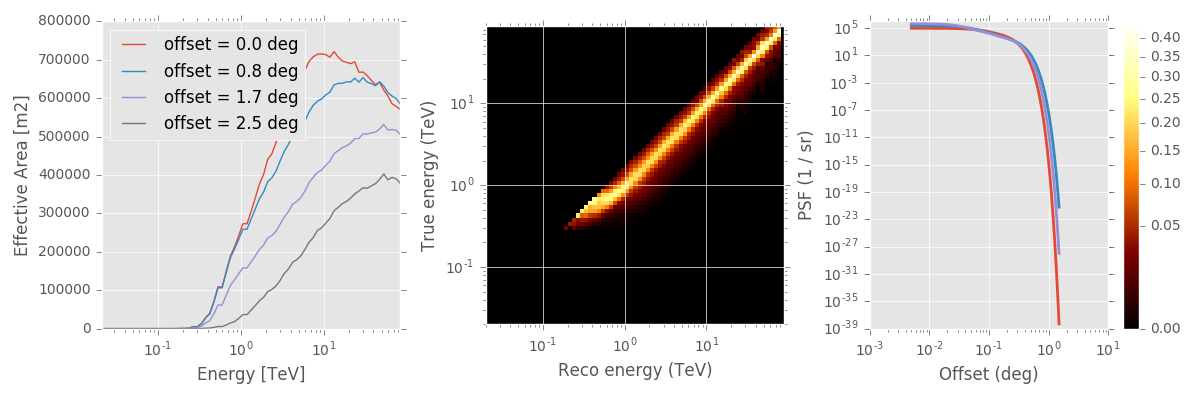
\includegraphics[width=\textwidth]{figures/iact-dl3}}
  \caption{Low-level example: IACT DL3}
\end{figure}

\begin{figure}[tb]
  \centerline{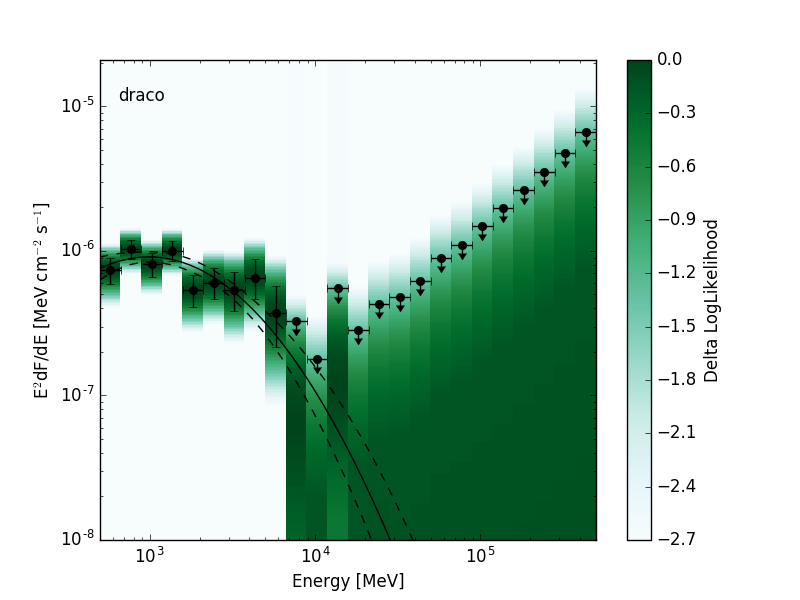
\includegraphics[width=\textwidth]{figures/llsed_hights}}
  \caption{High-level example: SED likelihood profiles}
\end{figure}


% % Table
\begin{table}[h]

\caption{Example table}
\label{tab:a}
\tabcolsep7pt\begin{tabular}{lcccc}
\hline
  & \tch{1}{c}{b}{Single\\ outlet}  & \tch{1}{c}{b}{Small\\ multiple\tabnoteref{t1n1}}  & \tch{1}{c}{b}{Large\\ multiple}  & \tch{1}{c}{b}{Total}   \\
\hline
1982 & 98 & 129 & 620    & 847\\
1987 & 138 & 176 & 1000  & 1314\\
1991 & 173 & 248 & 1230  & 1651\\
1998 & 200 & 300 & 1500\tabnoteref{t1n2}  & 2000\\
\hline
\end{tabular}
\tablenote[t1n1]{This is an example of first tablenote entry. This is an example of first tablenote entry.}
\tablenote[t1n2]{This is an example of second tablenote entry.}
\end{table}

